\section{Day 7: Separation Axioms and \texorpdfstring{$T_2$}{T2}/Hausdorff Spaces, More on Continuity (Sep. 24, 2024)}
Outfit of the day! Plaid outfit!
\begin{figure}[h]
    \centering
    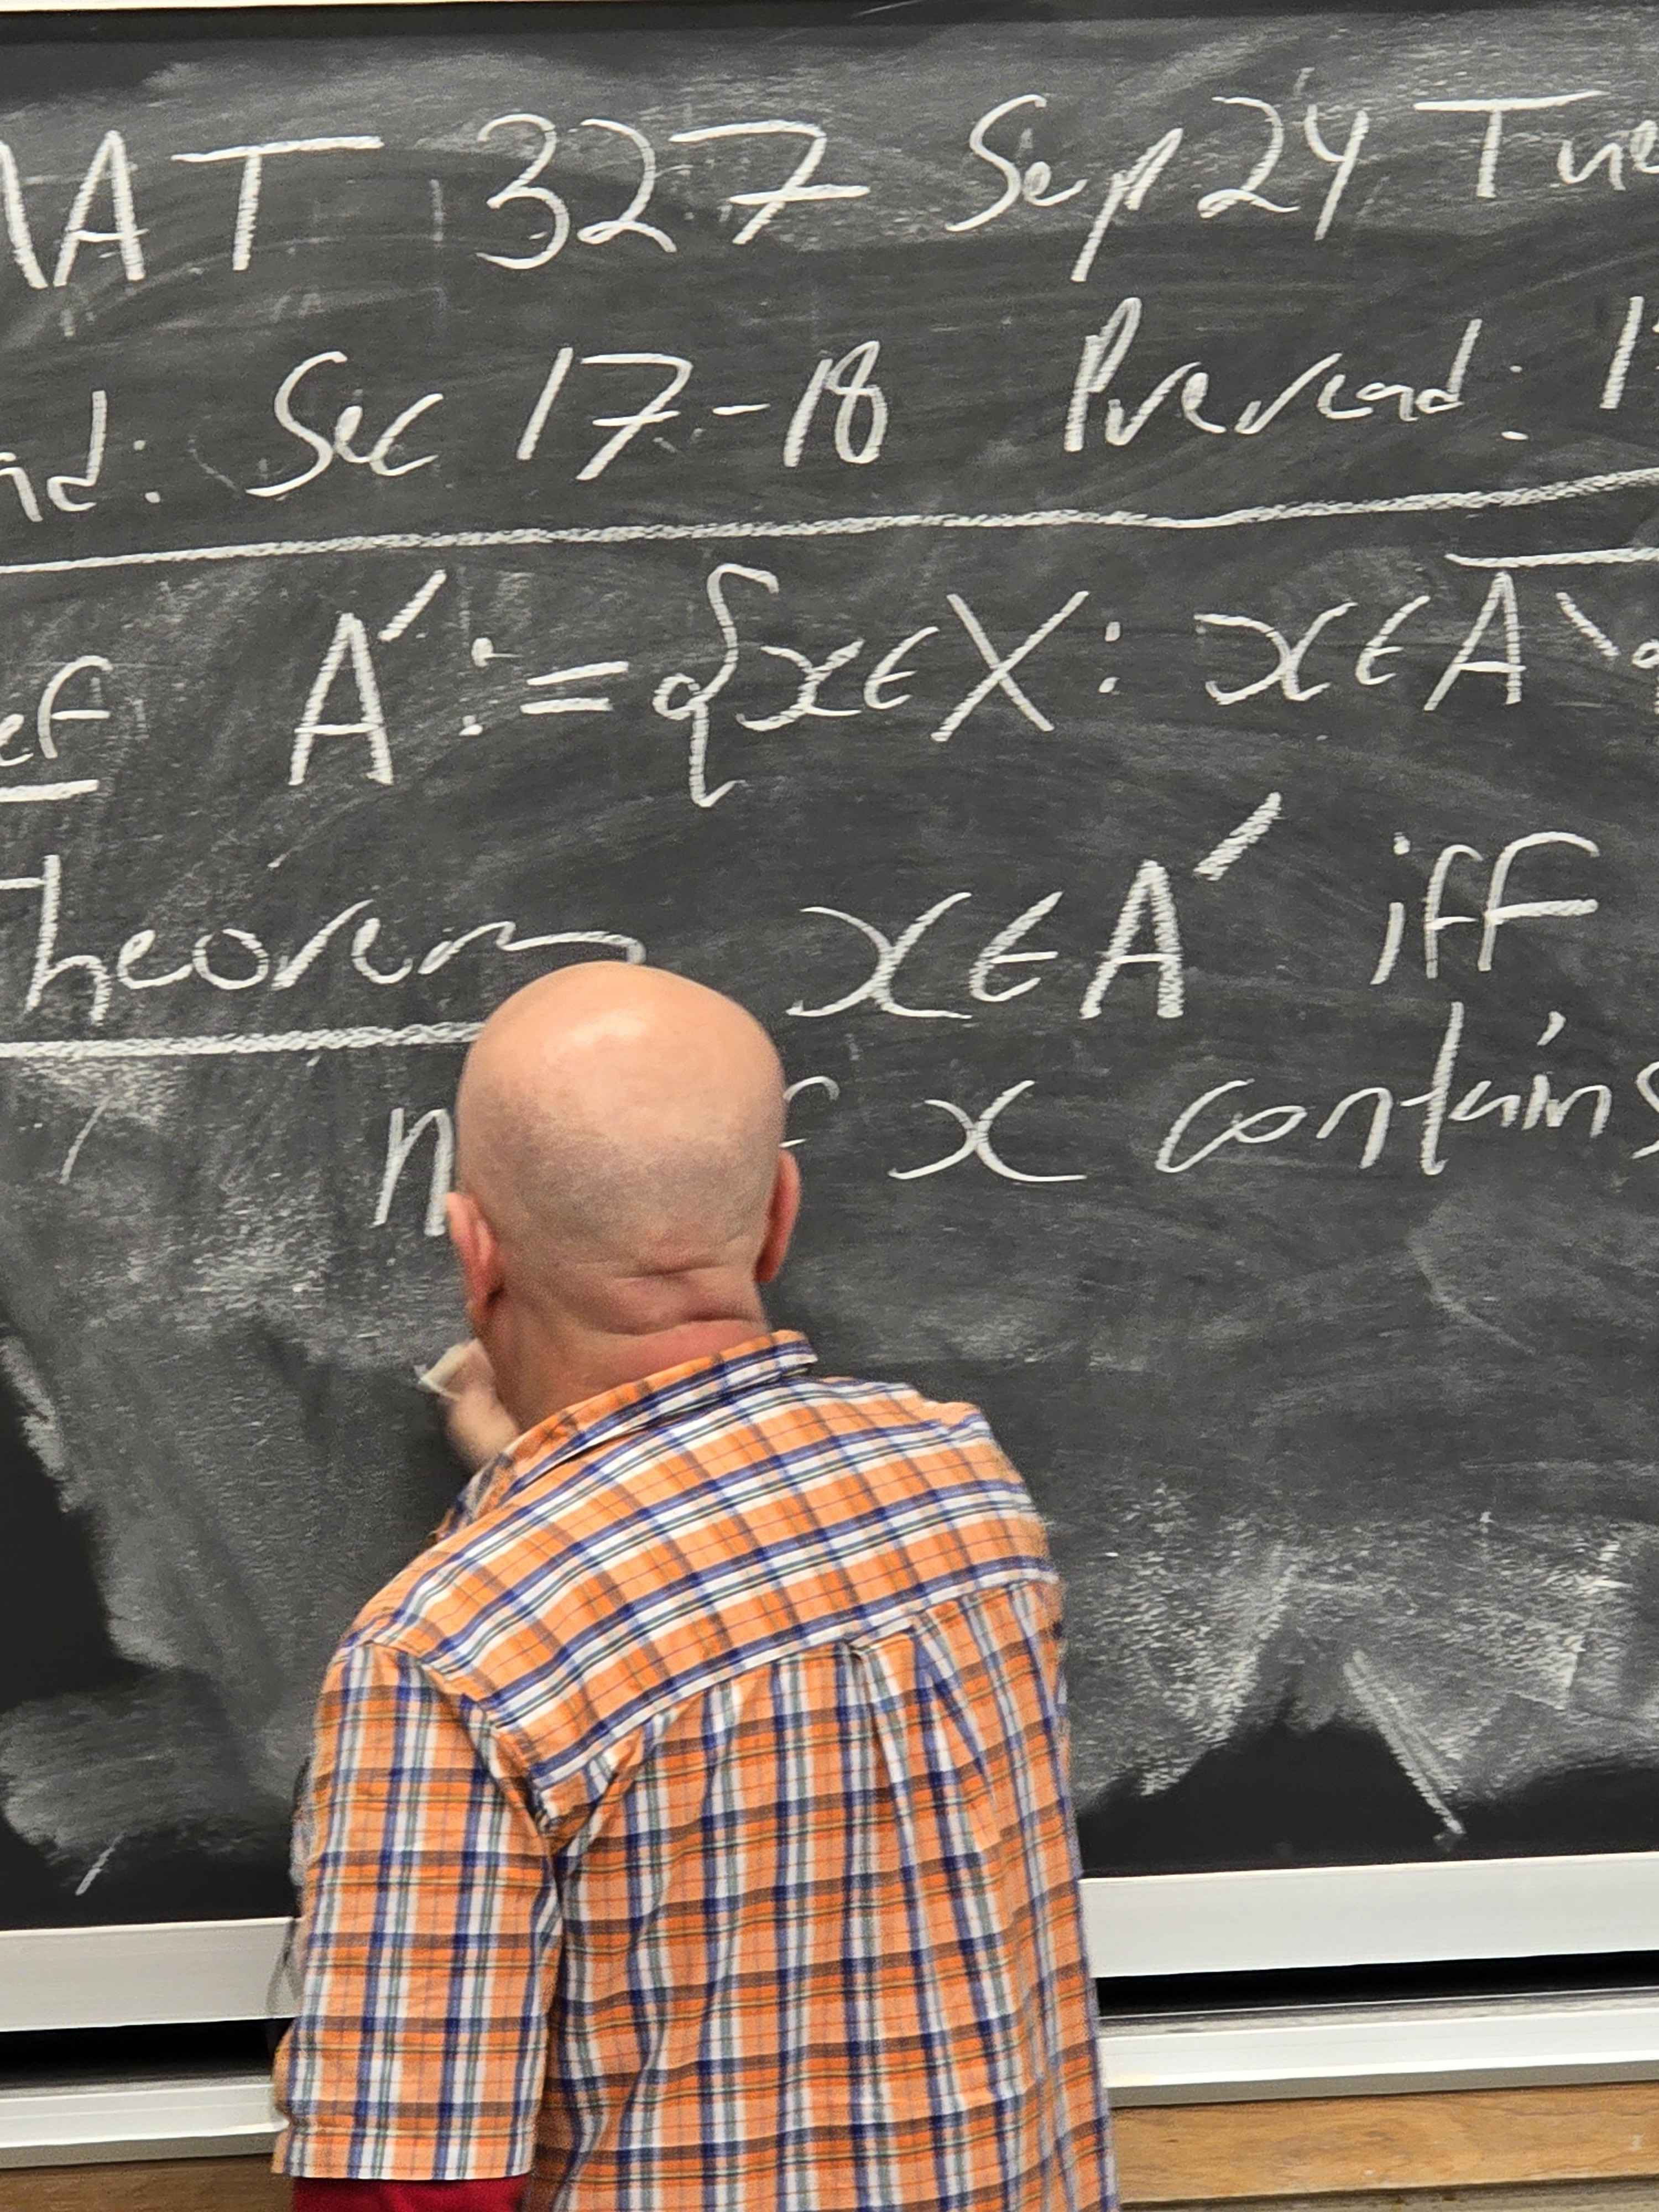
\includegraphics[scale=0.1]{MAT327 Notes/Dror Shirts/dror day 7 shirt.jpg}
\end{figure}

\noindent Recap of last lecture:
\begin{itemize}
    \item We define $A' := \{x \in X \mid x \in \overline{A \setminus \{x\}}$ to be the set of limit points of $A$ in $X$.
    \item We present a ``fheorem'' (read: false theorem): $x \in A'$ if and only if every neighborhood of $X$ contains infinitely many points of $A$, i.e.
    \[ x \in U \subset X \implies \abs{U \cap A} = \infty, \]
    where $U$ is open in $X$.
    \medskip\newline
    We expand on our ``froof'' from last time: indeed, if $U$ is a neighborhood of $X$, then as $x \in \overline{A \setminus \{x\}}$, we have that $U \cap (A \setminus \{x\}) \neq \emptyset$. Now, let us pick $a_1 \in U \cap (A \setminus \{x\})$, and consider $U_1 = U \setminus \{a_1\}$.
    \medskip\newline
    Since $U_1$ is a neighborhood of $x$, we have that $U_1 \cap \overline{A \setminus \{x\}} \neq \emptyset$, so we may pick $a_2 \in U_1 \cap \overline{A \cap \{x\}}$; then we consider $U_2$, etc... We argue by induction that there are infinitely many such points. Thus, there exists an infinite sequence of distinct points $\{a_i\}_{i \in \NN}$ in $U \cap A \setminus \{x\}$. \qed
    \medskip\newline
    This proof is in fact wrong because $U_1$ is not necessarily a neighborhood of $x$ (i.e., we don't know if $X \setminus \{a_1\}$ is open or not). For a blatant example, consider the trivial topology. Then $X \setminus \{a_1\}$ is obviously not open if $X$ is not a singleton.
\end{itemize}

\noindent To expand on our recap of last lecture, we introduce the \href{https://en.wikipedia.org/wiki/Separation_axiom}{separation axioms}.
\begin{itemize}
    \item[$T_1$:] A space $X$ is called $T_1$ if and only if, for all $x \in X$, $\{x\}$ is closed, and $X \setminus \{x\}$ is open, and for all $x, y \in X$ where $x \neq y$, we can find a neighborhood of $y$ that does not contain $x$, i.e. $\exists U$ open in $X$ such that $x \in U$ but $y \not\in U$. These three conditions are equivalent to each other; though usually, it is useful to just identify it as singletons being closed, or their complements being open.
    \medskip\newline
    In particular, our ``froof'' from earlier holds if $X$ is $T_1$ (i.e., any singleton is closed, and so the union of singletons are closed).
    \item[$T_2$:] We say a space $X$ is $T_2$ (aka Hausdorff or \textit{separated}) if, for all $x, y \in X$ where $x \neq y$, then there exists open sets $U_1, U_2$ in $X$ such that $U_1 \cap U_2 = \emptyset$.
    \begin{exercise}
        Show that if $x_1, \dots, x_n \in X$, then there exists open sets $U_1, \dots, U_n$ such that $x_i \in U_i$ and $i \neq j \implies U_i \cap U_j = \emptyset$.
    \end{exercise}
    \begin{simpleclaim}
        We claim that if $X$ is $T_2$, then it is also $T_1$.
    \end{simpleclaim}
    This is clear by picking neighborhoods $U_1, U_2$ for $x, y \in X$ where $x \neq y$, such that $U_1 \cap U_2 = \emptyset$. Clearly, $U_1$ does not contain $y$, and $U_2$ does not contain $x$. \qed
    \begin{simpleclaim}
        In a $T_2$ space, any sequence has at most one limit.
    \end{simpleclaim}
    \noindent In particular, we define sequence convergence as follows; if $\{a_n\}_{n \in \NN} \in X$, then we say that $a_n$ converges to $a \in X$, i.e. $a_n \to a$ as $n \to \infty$, or $\lim_{n \to \infty} a_n = a$, if for every neighborhood $U$ of $a$, there exists $N$ such that $n > N$ implies $a_n \in U$.
    \medskip\newline
    We now prove claim 7.3. Assume $\{a_n\}_{n \in \NN}$ is a sequence that converges to $a$ and $a'$, i.e. $a_n \to a$ and $a_n \to a'$. Then by $T_2$, there exists neighborhoods $U, U'$ of $a, a'$ respectively such that $U \cap U' = \emptyset$. Then, let us pick a large enough $N$ such that $n > N \implies a_n \in U$, and $N'$ large enough such that $n > N' \implies a_n \in U'$. Then just consider $n = \max\{N, N'\} + 1$, then $a_n \in U$ and $U'$ at once, while $U \cap U' = \emptyset$. This is contradictory, and so we are done. \qed
\end{itemize}

\noindent We now make the following claim.
\begin{simpleclaim}
    We claim that a subspace of a $T_2$ space is $T_2$, and that the product of $T_2$ spaces is also $T_2$.
\end{simpleclaim}
\noindent We start by proving the claim on products\footnote{im not including the froof from class because i think it's kind of immediate, sorry. also i didn't catch it entirely so oh well}. Suppose $X, Y$ are $T_2$, and let us have $a_1, a_2 \in X \times Y$ where $a_1 = (x_1, y_1) \neq (x_2, y_2) = a_2$. Then $x_1 \neq x_2$ or $y_1 \neq y_2$. Without loss of generality, suppose $y_1 \neq y_2$. Then there exists neighborhoods $V_1, V_2$ in $Y$ of $y_1, y_2$ respectively, where $V_1 \cap V_2 = \emptyset$. Then we see that $X \times V_1$ and $X \times V_2$ are suitable choices of neighborhoods for $a_1, a_2$ to conclude that $X \times Y$ is $T_2$.

\newpage
\noindent We now move onto a different topic.
\begin{simplethm}
    Given $f : X \to Y$, we have that the following are equivalent:
    \begin{enumerate}[label=(\alph*)]
        \item $f$ is continuous.
        \item $f(\overline{A}) \subset \overline{f(A)}$, i.e. $f$ maps the closure of $A$ into the closure of $f(A)$.
        \item If $B \subset Y$ is closed, then $f^{-1}(B)$ is closed.
        \item For all $x_0 \in X$, if $V$ is a neighborhood of $f(x_0)$, then there is a negihborhood $U$ of $x_0$ such that $f(U) \subset V$.
    \end{enumerate}
\end{simplethm}
\noindent Note that we have already proven that (a) if and only if (c), (a) iff (d), and we will prove that (a) implies (b) and (b) implies (c) on Thursday.